\chapter[Aplicação]{Aplicação}\label{sec-aplicacoes}

Os dados utilizados neste capítulo provêm do experimento \emph{Low Carbon London} \cite{schofield2015lcl}, conduzido pela \emph{UK Power Networks} entre 2011 e 2014.
A atribuição de tarifas variáveis com a hora do dia a domicílios residenciais, e o acompanhamento do consumo elétrico resultante correspondem, em termos precisos, ao problema que motivou os exemplos dos capítulos anteriores.
Aplicamos a esses dados, os estimadores do Capítulo \ref{sec-metodologia}.

\section{Aprofundamento do problema}\label{sec-aplicacoes-problema}

A cada domicílio participante foi atribuída uma de duas modalidades tarifárias: a tarifa padrão, de preço fixo independentemente do horário de consumo, e a tarifa dinâmica (\emph{time-of-use}, ToU), cujos preços variam ao longo do dia, com valores mais elevados nos horários de pico. 
O consumo elétrico foi registrado em intervalos de 30 minutos entre 2011 e 2014, mas a análise restringe-se ao ano civil de 2013, período de vigência ativa da tarifa ToU, produzindo \(T = 17.520\) observações por unidade amostral.
São incluídos apenas os domicílios com leituras cobrindo esse período por completo, condição que, combinada às exclusões descritas a seguir, determina a amostra final de \(N = 5.095\) domicílios.

Os domicílios são classificados segundo o sistema ACORN (\emph{A Classification of Residential Neighbourhoods}, em português: Classificação de Bairros Residenciais), segmentação socioeconômica baseada no censo britânico de 2011 que agrupa residências por perfil de renda e características demográficas. 
As categorias consolidadas utilizadas na análise são \emph{Affluent} (Afluente, \(n = 1.970\)), \emph{Comfortable} (Confortável, \(n = 1.407\)), \emph{Adversity} (Adversidade, \(n = 1.674\)) e \emph{ACORN-U} (\(n = 44\)), que entram no modelo como covariáveis pré-tratamento \(\mathbf{X}_i\).
Uma quinta categoria, \emph{ACORN-}, teve unidades excluídas da análise porque os domicílios nessa classificação pertenciam integralmente ao grupo dos tratados, o que violaria a suposição de positividade (Seção \ref{sec-inferencia-causal}). 
Um dos domicílios, com identificador MAC005565, foi removido individualmente por apresentar série corrompida.

Neste enquadramento, \(A_i = 1\) indica que o domicílio \(i\) recebeu a tarifa ToU e \(A_i = 0\) que recebeu a tarifa padrão. 
O desfecho \(Y_i(t)\) é a curva de consumo elétrico do domicílio \(i\) no instante \(t \in \mathcal{T}\) (nesta aplicação, os desfechos são observados somente após a atribuição do tratamento). 
O interesse está em estimar o \(\mathrm{FATE}\), \(\theta(t) = \mathbb{E}[Y_i^{(1)}(t) - Y_i^{(0)}(t)]\), a diferença média entre a curva de consumo que cada domicílio apresentaria sob ToU e a que apresentaria sob tarifa padrão.

Os domicílios participantes aderiram voluntariamente ao experimento, e as tarifas foram distribuídas por aleatorização estratificada segundo o grupo ACORN, justificando a ignorabilidade condicional em \(\mathbf{X}_i\) e a inclusão dessas categorias como covariáveis no modelo. 
As demais condições para identificabilidade são igualmente plausíveis (considerando que garantimos a positividade com a retirada do grupo \emph{ACORN-}). 
A tarifa de cada domicílio é bem definida (consistência) e o consumo de um domicílio não depende da tarifa atribuída aos vizinhos (ausência de interferência). 
O recrutamento por adesão implica, porém, que as estimativas descrevem o efeito causal para o perfil de domicílio que adere a programas dessa natureza, e não para o conjunto geral de domicílios londrinos.

\section{Análise exploratória}\label{sec-aplicacoes-exploratoria}

Antes da estimação formal, convém examinar a estrutura dos dados observados.
Os padrões de consumo de cada grupo, visíveis diretamente nas séries brutas, fornecem o referencial necessário para interpretar as estimativas do \(\mathrm{FATE}\) e do \(\mathrm{CFATE}\) apresentadas na seção seguinte.

A Figura \ref{fig:lcl-consumo-anual} apresenta a média diária do consumo registrado, calculada separadamente para cada grupo tarifário.
O padrão sazonal é pronunciado, com consumo mais alto no inverno britânico, mínimos em julho e agosto, e recuperação no segundo semestre.
Olhando para os dados, sem qualquer ajuste para possíveis confundidoras, vemos que os domicílios com tarifa padrão consomem, em média, mais do que os com tarifa dinâmica em praticamente todos os dias do ano, com diferenças mais expressivas nos meses frios.
As oscilações de alta frequência visíveis nas séries refletem o ciclo semanal, com consumo mais elevado nos fins de semana.

\begin{figure}[htbp]
    \centering
    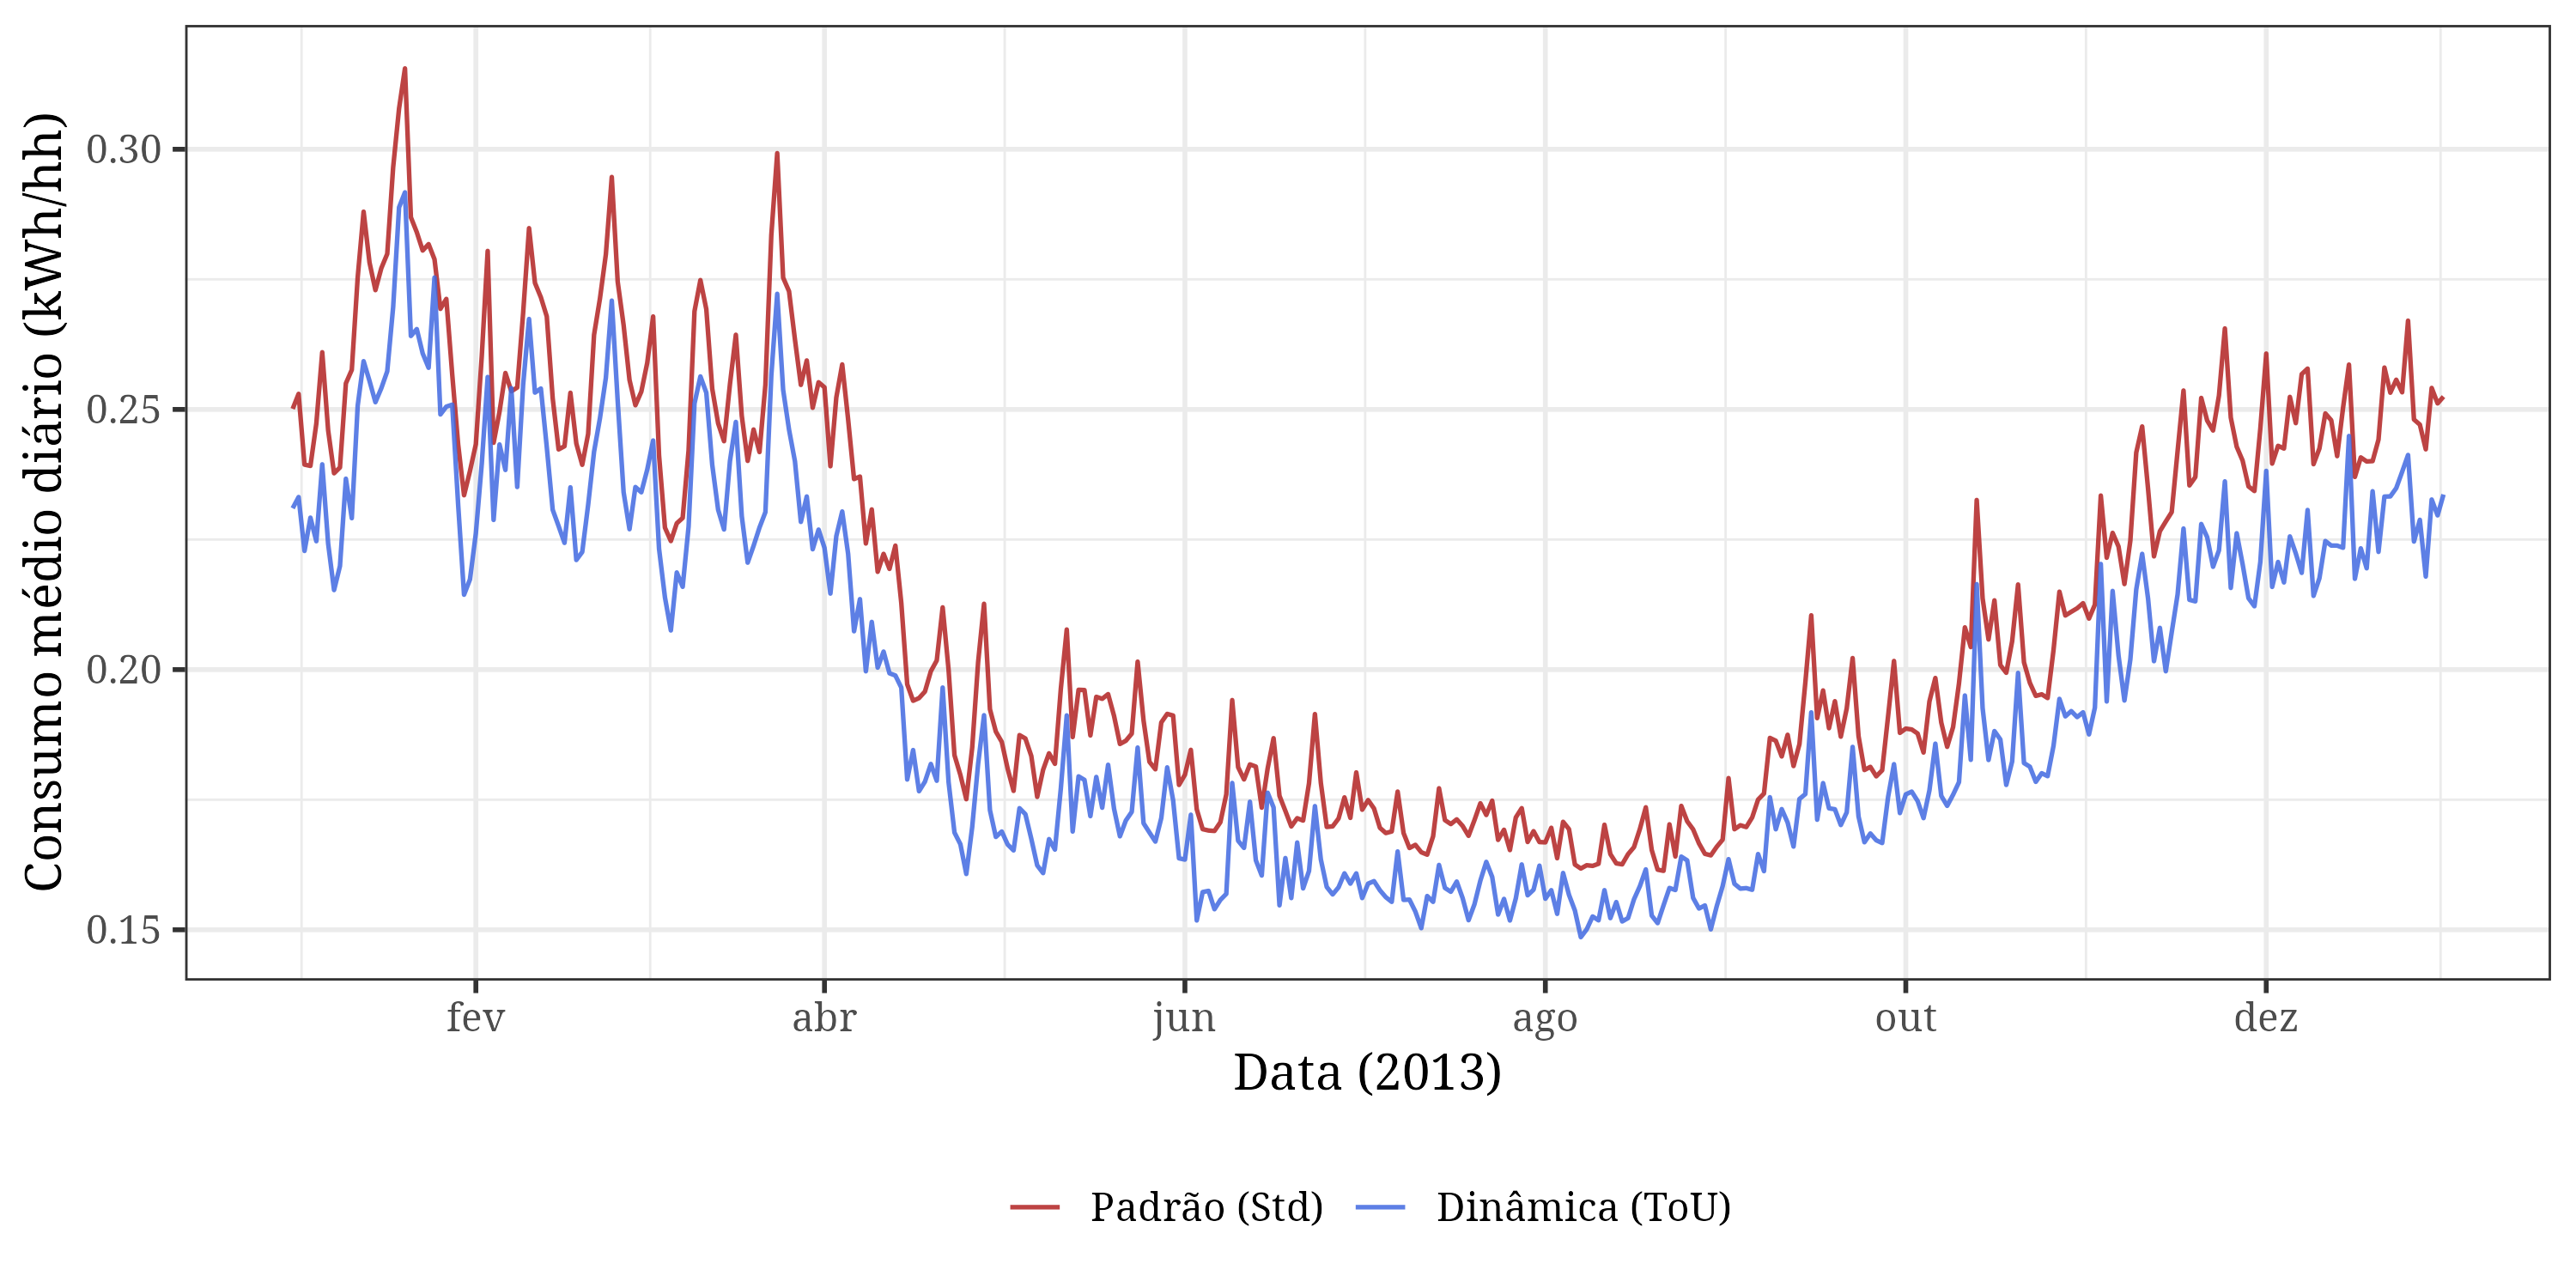
\includegraphics[width=0.9\textwidth]{../../fate-fda-application/low_carbon_energy/output/lcl_final/plots/main_text/annual_mean_by_group}
    \caption{Consumo médio diário por grupo tarifário ao longo de 2013, calculado sobre os domicílios com leitura disponível em cada dia, sem ajuste causal.}
    \label{fig:lcl-consumo-anual}
\end{figure}

A Figura \ref{fig:lcl-perfil-diario} apresenta o consumo médio por intervalo de 30 minutos, desagregado por trimestre e grupo tarifário.
O padrão ao longo do dia é dominado por um pico noturno entre 19h e 21h, mais pronunciado nos meses frios.
No verão (Q3), esse pico se atenua e os grupos se aproximam.

\begin{figure}[htbp]
    \centering
    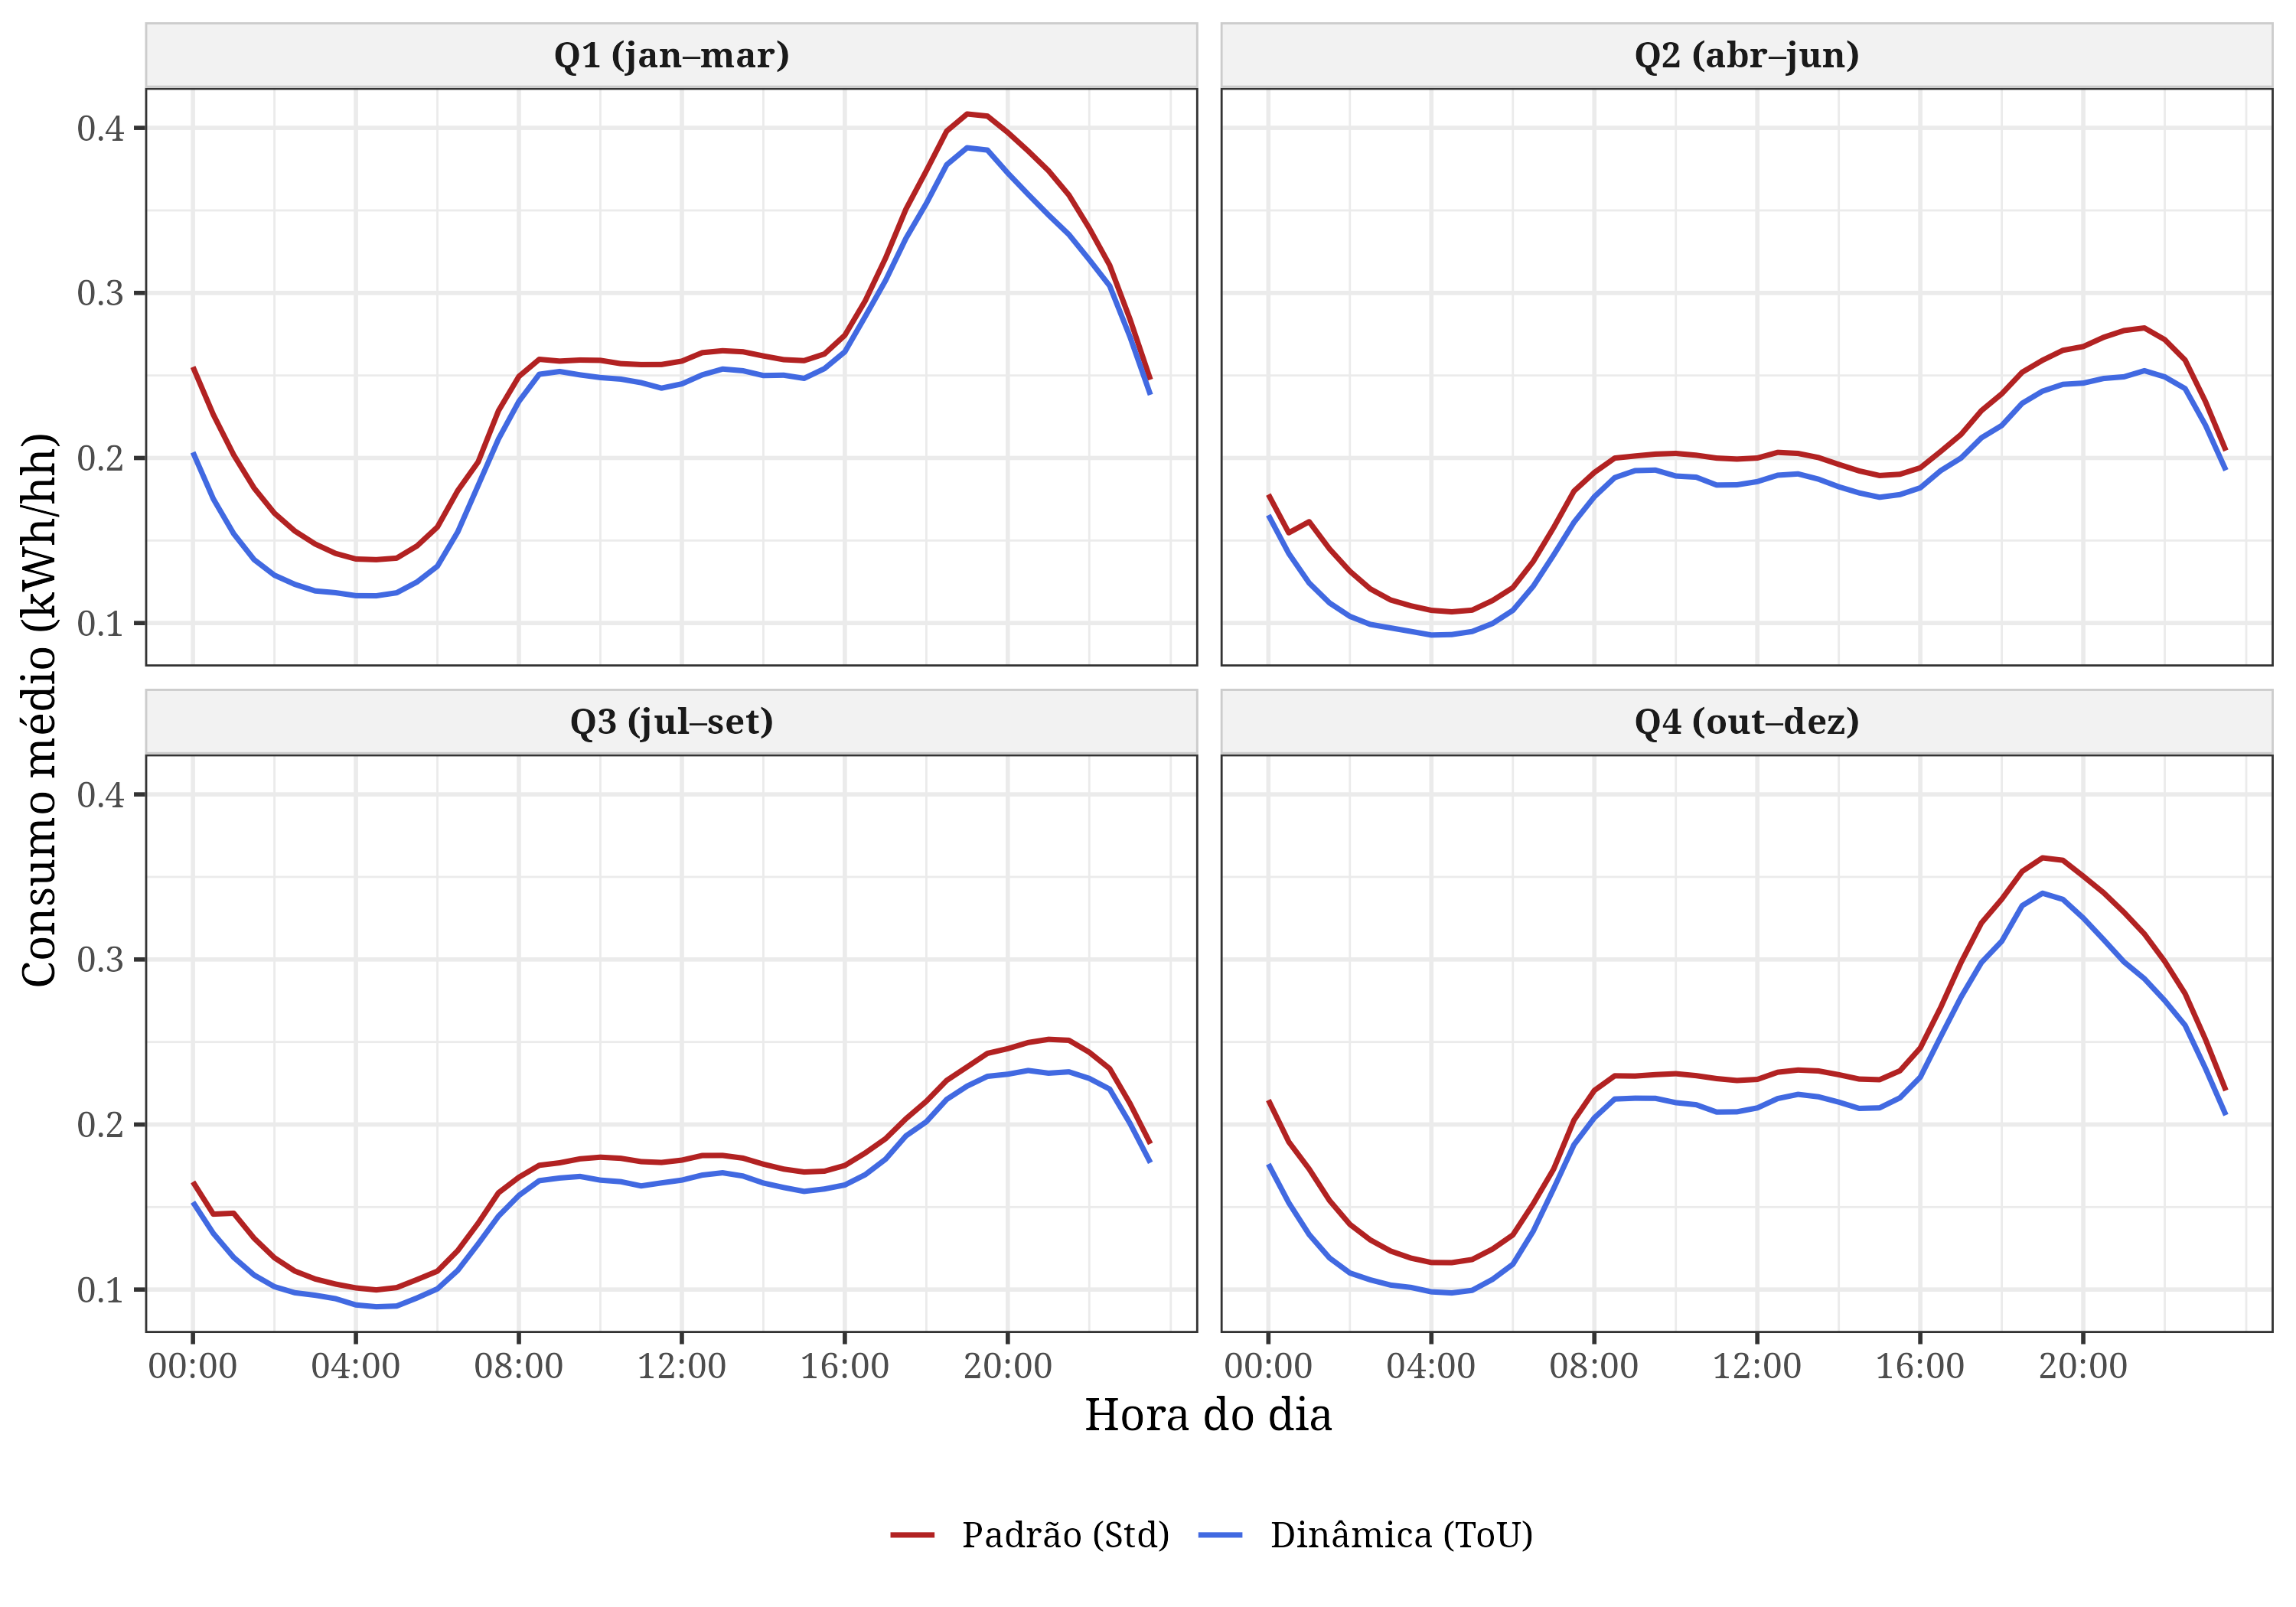
\includegraphics[width=0.9\textwidth]{../../fate-fda-application/low_carbon_energy/output/lcl_final/plots/main_text/intraday_by_season}
    \caption{Consumo médio por intervalo de 30 minutos, desagregado por trimestre e grupo tarifário, sem ajuste causal.}
    \label{fig:lcl-perfil-diario}
\end{figure}

A decomposição da diferença bruta de consumo por grupo ACORN revela heterogeneidade considerável.
A Figura \ref{fig:lcl-diff-acorn-diario} apresenta, para cada categoria, a diferença entre o consumo médio do grupo ToU e o do grupo padrão ao longo do dia.
\emph{Affluent} e \emph{Comfortable} reduzem o consumo sob a tarifa dinâmica em praticamente todos os horários, com a redução mais pronunciada no pico vespertino.
\emph{Adversity} apresenta diferença próxima de zero ao longo do dia, sugerindo menor resposta ao incentivo tarifário.
\emph{ACORN-U} exibe comportamento atípico, com diferenças positivas expressivas no período da tarde e da noite. Dada a pequena dimensão desse grupo (\(n = 44\)), o resultado deve ser interpretado com cautela.

\begin{figure}[htbp]
    \centering
    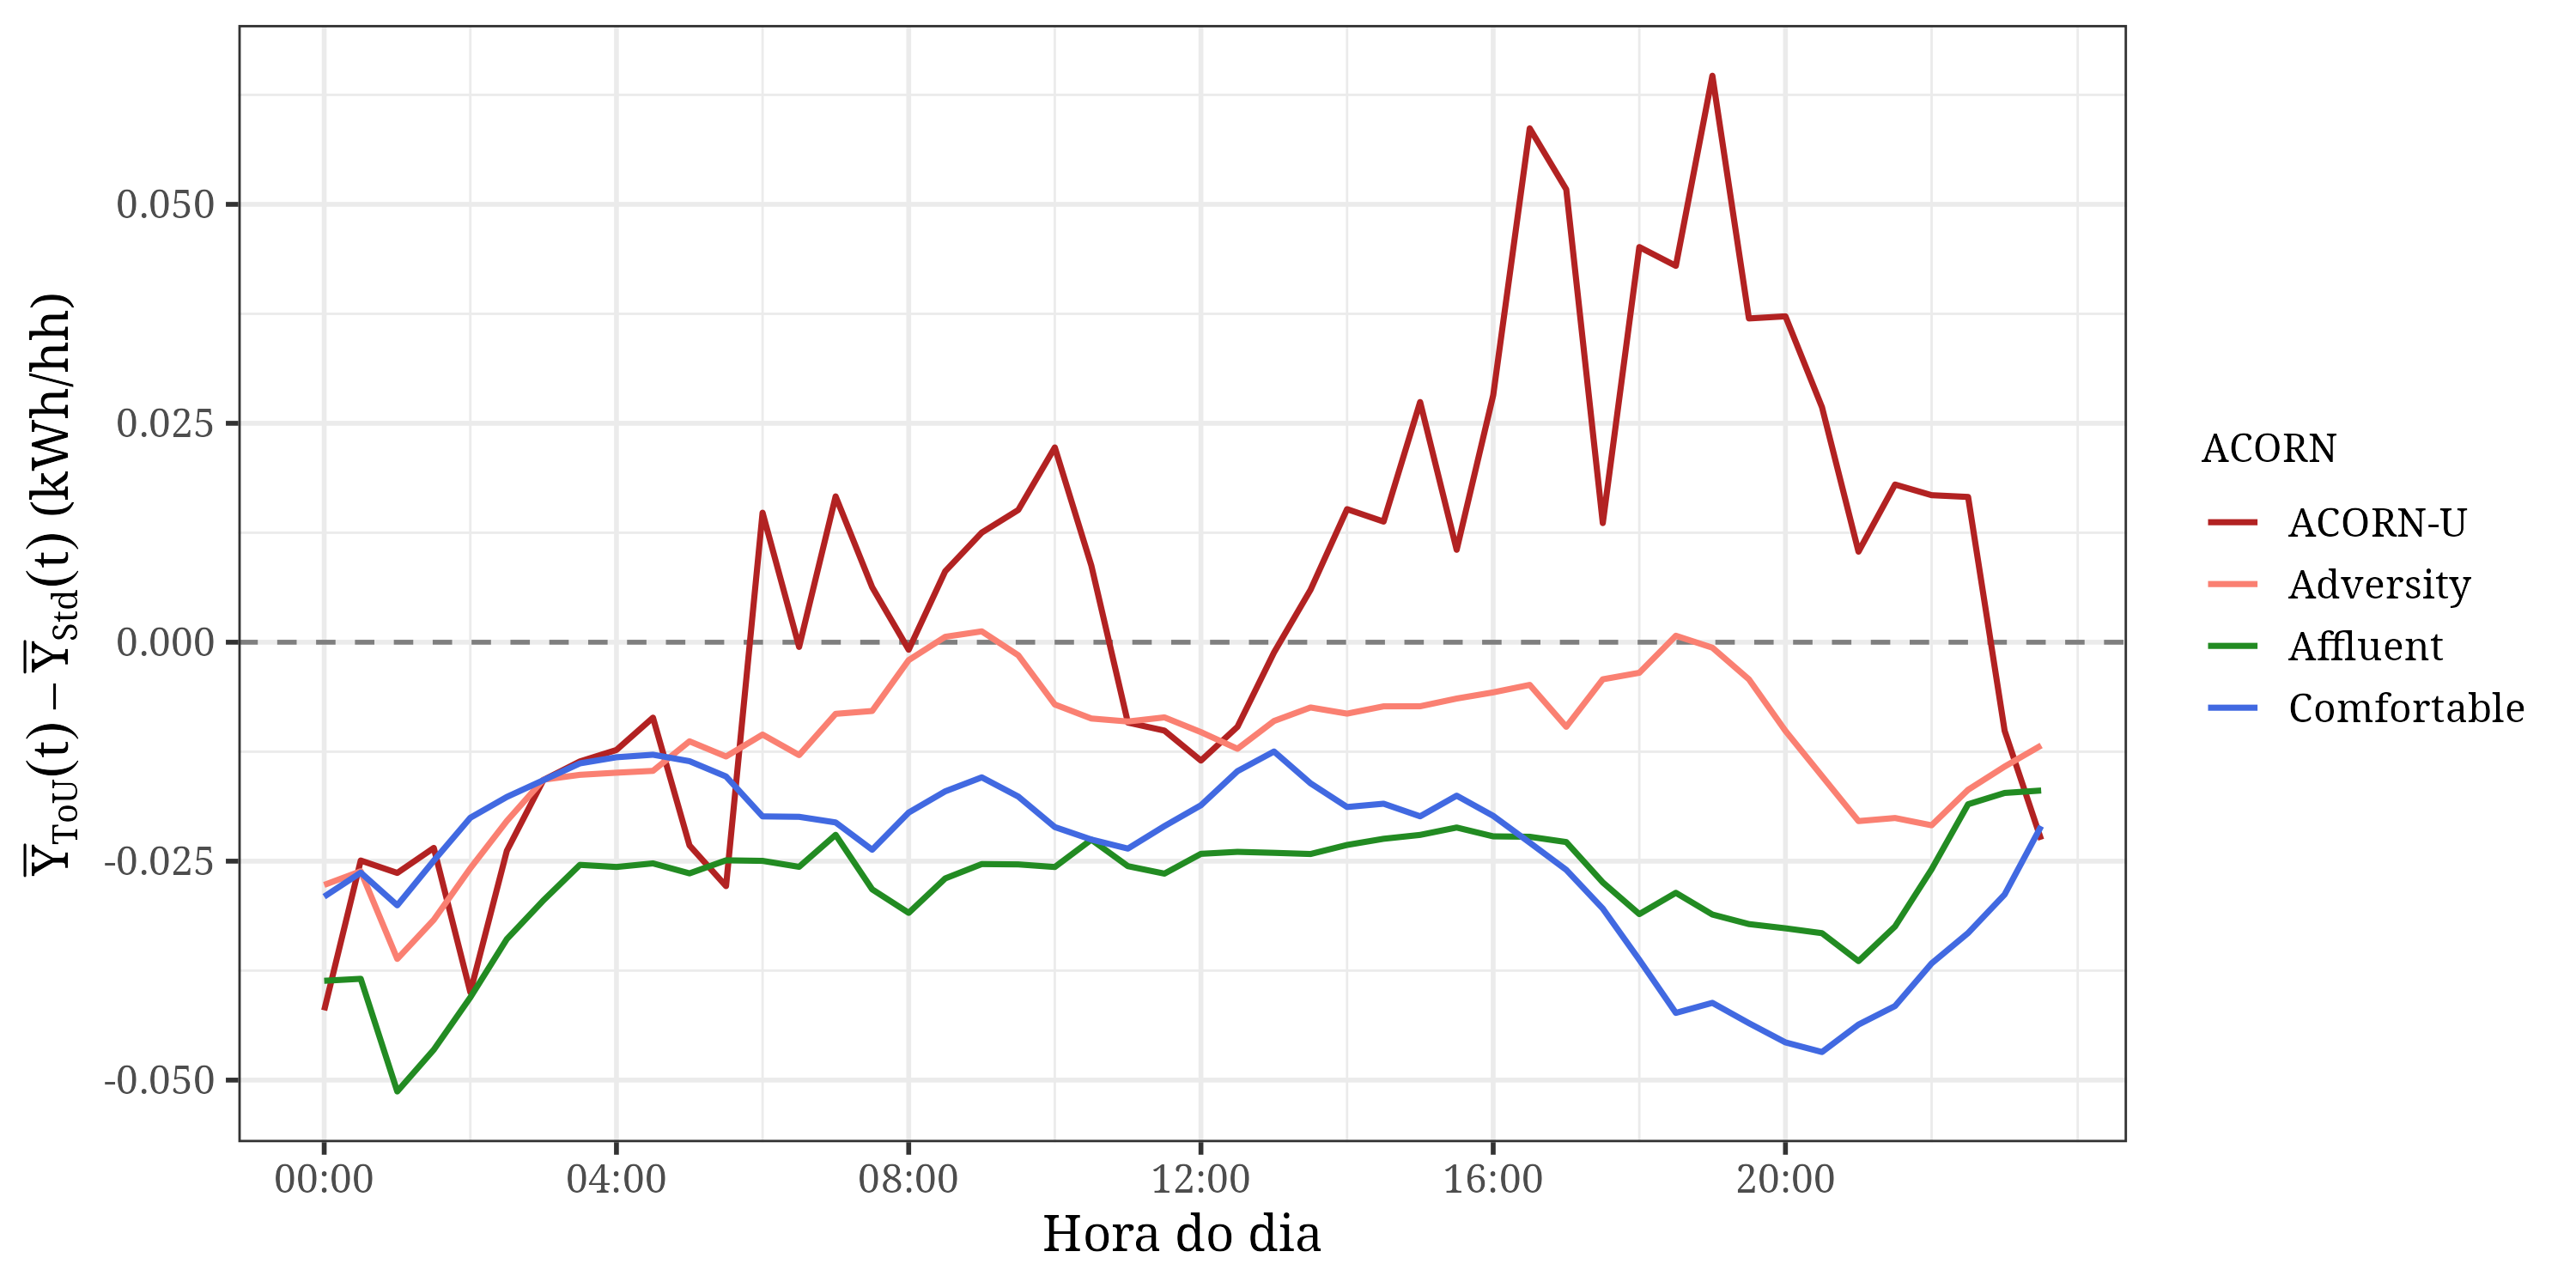
\includegraphics[width=0.9\textwidth]{../../fate-fda-application/low_carbon_energy/output/lcl_final/plots/main_text/fate_raw_by_acorn_intraday}
    \caption{Diferença bruta de consumo \(\bar{Y}_{\mathrm{ToU}}(t) - \bar{Y}_{\mathrm{Std}}(t)\) por grupo ACORN ao longo do dia, sem ajuste causal.}
    \label{fig:lcl-diff-acorn-diario}
\end{figure}

Finalmente, vale pontuar que cerca de 78\% dos domicílios registram ao menos uma leitura ausente ao longo do ano, decorrente de falhas operacionais nos medidores. Esse mecanismo parece ser independente do padrão de consumo do domicílio (e assumiremos tal independência). A proporção de domicílios com tarifa ToU entre os que apresentam ao menos uma falta é de 19,8\%, muito próxima à proporção global de 20,4\%. 
As ausências também se distribuem de forma dispersa ao longo do ano, sem concentração nos horários de pico.

O Apêndice \ref{ap-aplicacoes} complementa esta breve análise exploratória com um mapa de calor do consumo médio por semana e hora do dia, com o envelope funcional das séries observadas, com os gráficos de distribuição das leituras ausentes e com o gráfico de diferença média do consumo entre os grupos de tratamento e controle, por ACORN, ao longo do ano (ainda sem controlar por causalidade).

\section{Estimação do efeito causal e discussão}\label{sec-aplicacoes-resultados}

Para estimar o efeito da tarifa dinâmica sobre as curvas de consumo, era necessário suavizar as séries de todos os \(N = 5.095\) domicílios. 
Para isso, utilizamos o \texttt{rLifting} nos modos \emph{offline} e \emph{online}, o que nos permitiu comparar as estimativas causais obtidas sob as duas abordagens de pré-processamento.

Em ambos os modos, empregamos o esquema de ondaletas de Haar, limiarização universal e encolhimento SCAD, com o número de níveis \(J\) e os coeficientes \(\alpha\) e \(\beta\) da regra de limiarização selecionados por minimização do SURE mediano em uma amostra de 30 domicílios. 
No modo \emph{online}, definimos janelas móveis de tamanho \(W = \max(337,\, 16 \times 2^{J})\).

Com as curvas suavizadas, aplicamos os estimadores das Seções \ref{sec-estimador-offline} e \ref{sec-estimador-online}, com bandas de confiança simultâneas a 95\% pelo procedimento da Seção \ref{sec-bootstrap-ic} e \(\mathrm{CFATE}\) conforme a Seção \ref{sec-cfate}.

A Figura \ref{fig:lcl-fate-intradiario} apresenta o perfil intradiário médio do \(\hat{\theta}(t)\), comparando a diferença bruta e as estimativas ajustadas por ACORN nos dois modos de pré-processamento. 
Todas as curvas são negativas em todos os horários, indicando que domicílios sob tarifa dinâmica apresentaram consumo inferior ao contrafactual sob tarifa padrão ao longo de todo o dia. 
O efeito é mais pronunciado nas primeiras horas da madrugada, com vale próximo a \(-0{,}04\) kWh/hh, e reaparece no período noturno, por volta das 21h. 
Os estimadores \emph{offline} e \emph{online} produzem curvas praticamente sobrepostas. 
O ajuste por ACORN resulta em estimativas ligeiramente mais negativas do que a diferença bruta. 

\begin{figure}[htbp]
    \centering
    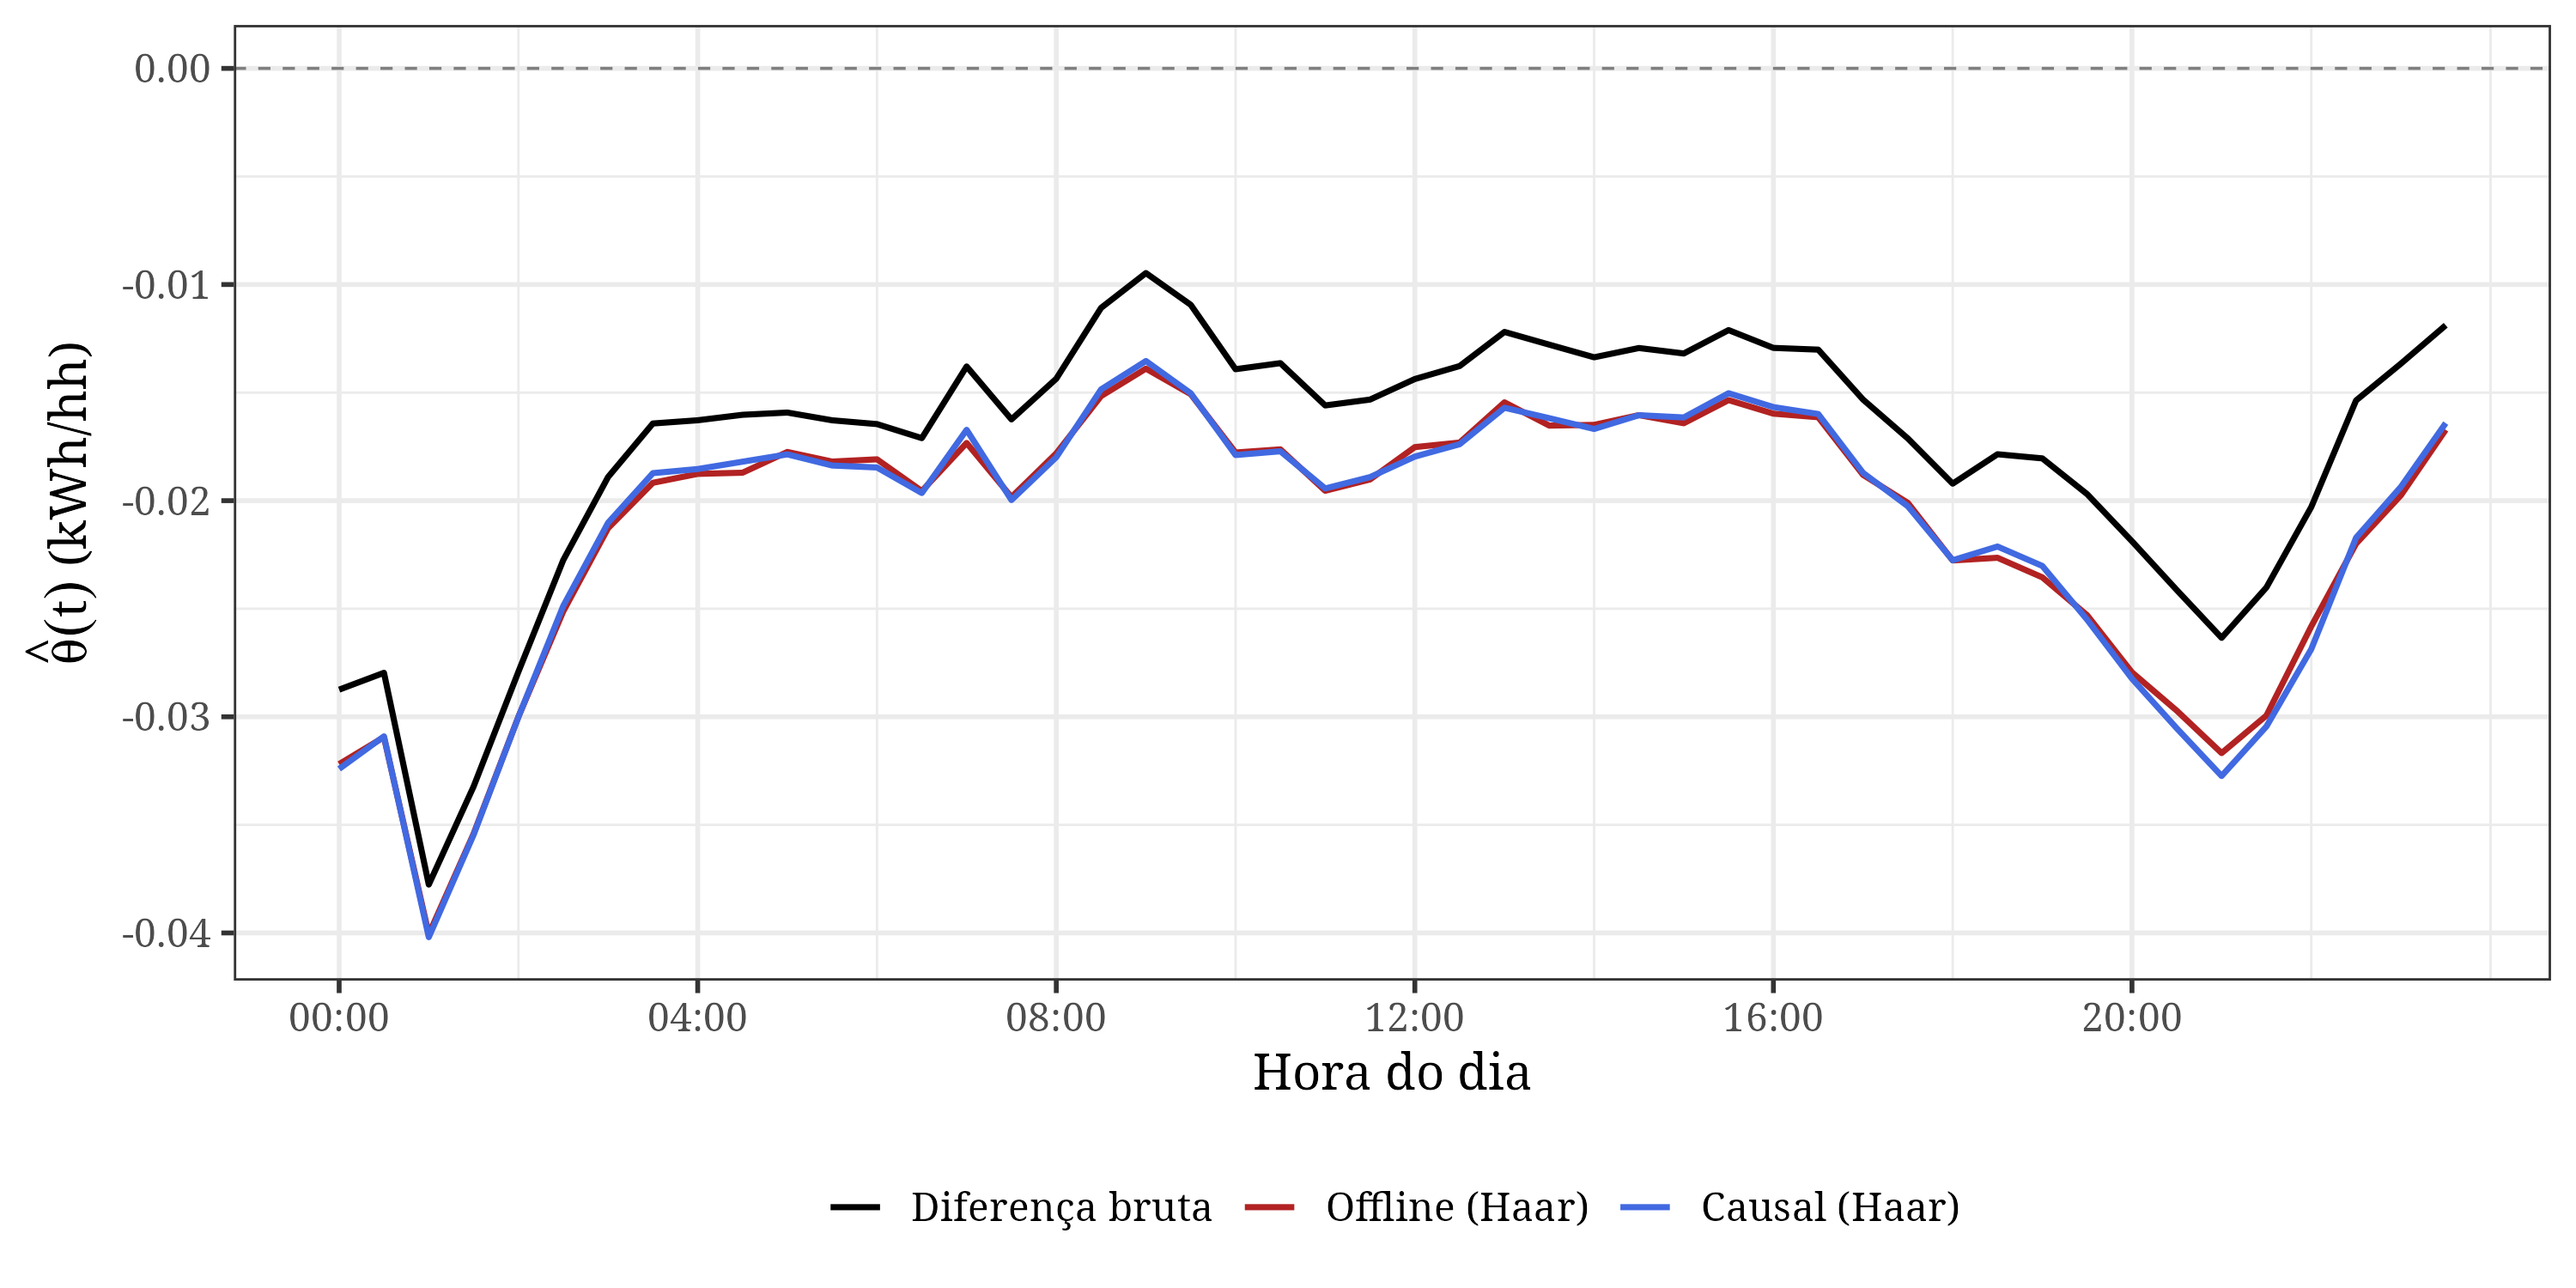
\includegraphics[width=0.9\textwidth]{../../fate-fda-application/low_carbon_energy/output/lcl_final/plots/main_text/fate_intraday_comparison}
    \caption{Perfil intradiário médio do \(\hat{\theta}(t)\): diferença bruta, estimativa \emph{offline} (Haar) e estimativa \emph{online} (Haar), agregadas por intervalo de 30 minutos ao longo de 2013.}
    \label{fig:lcl-fate-intradiario}
\end{figure}

A Figura \ref{fig:lcl-fate-bandas} apresenta \(\hat{\theta}(t)\) na resolução nativa de 30 minutos, nos dois modos de pré-processamento.
A curva oscila com alta frequência e fica abaixo de zero ao longo de todo o ano, mas as bandas simultâneas a 95\% cruzam zero em praticamente todos os instantes, de modo que o sinal do efeito em cada ponto isolado permanece incerto.
A Figura \ref{fig:lcl-cfate-anual} mostra como esse sinal se consolida.
O \(\mathrm{CFATE}\) decresce monotonicamente e encerra 2013 em \(-372\) kWh/hh\footnote{A unidade kWh/hh (quilowatt-hora por domicílio) indica que o valor é a média por domicílio, não um total agregado. As leituras \(Y_i(t)\) registram energia em kWh por intervalo de 30 minutos; o \(\mathrm{CFATE}\) acumula as diferenças ao longo dos \(T = 17.520\) intervalos do ano.} [IC 95\%: \(-534\); \(-209\)].
O limite superior da banda simultânea a 95\% fica abaixo de zero desde os primeiros meses, de modo que o efeito acumulado é estatisticamente discernível durante a maior parte do ano.
Os modos \emph{offline} e \emph{online} produzem trajetórias praticamente idênticas.

\begin{figure}[htbp]
    \centering
    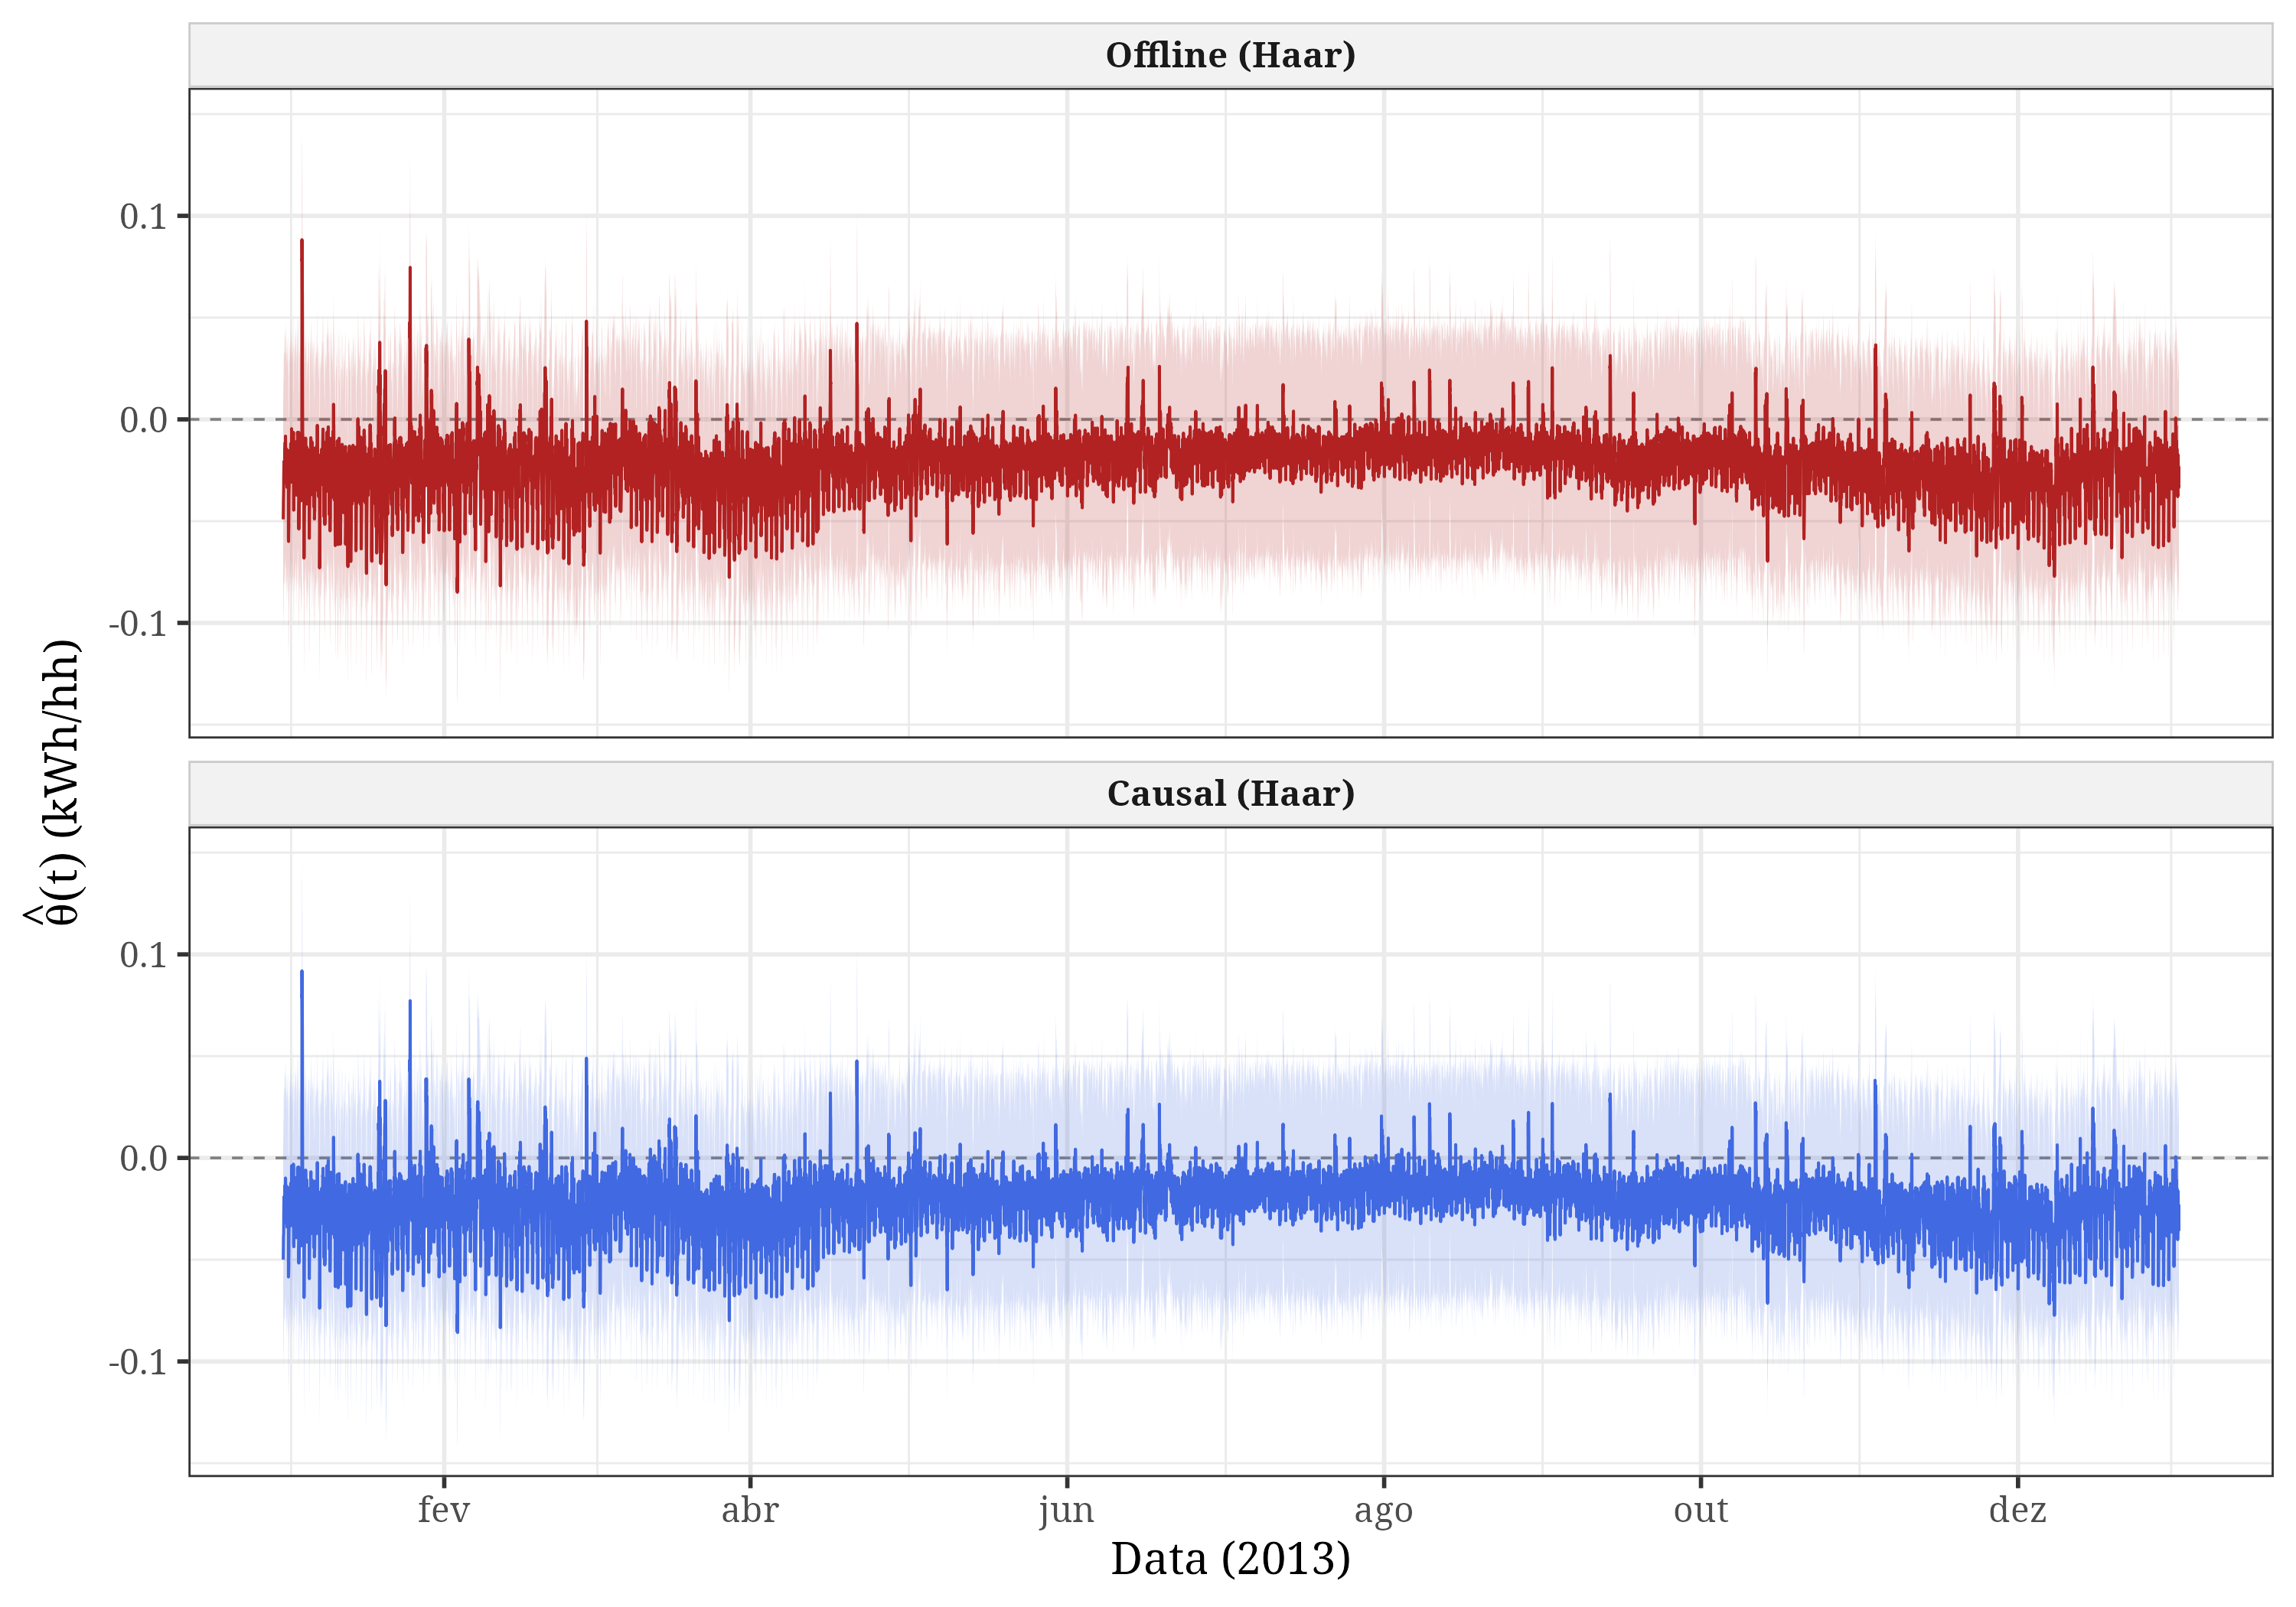
\includegraphics[width=0.9\textwidth]{../../fate-fda-application/low_carbon_energy/output/lcl_final/plots/main_text/fate_bands}
    \caption{Estimativa \(\hat{\theta}(t)\) na resolução de 30 minutos com bandas de confiança simultâneas a 95\%, nos modos \emph{offline} e \emph{online} (Haar).}
    \label{fig:lcl-fate-bandas}
\end{figure}

\begin{figure}[htbp]
    \centering
    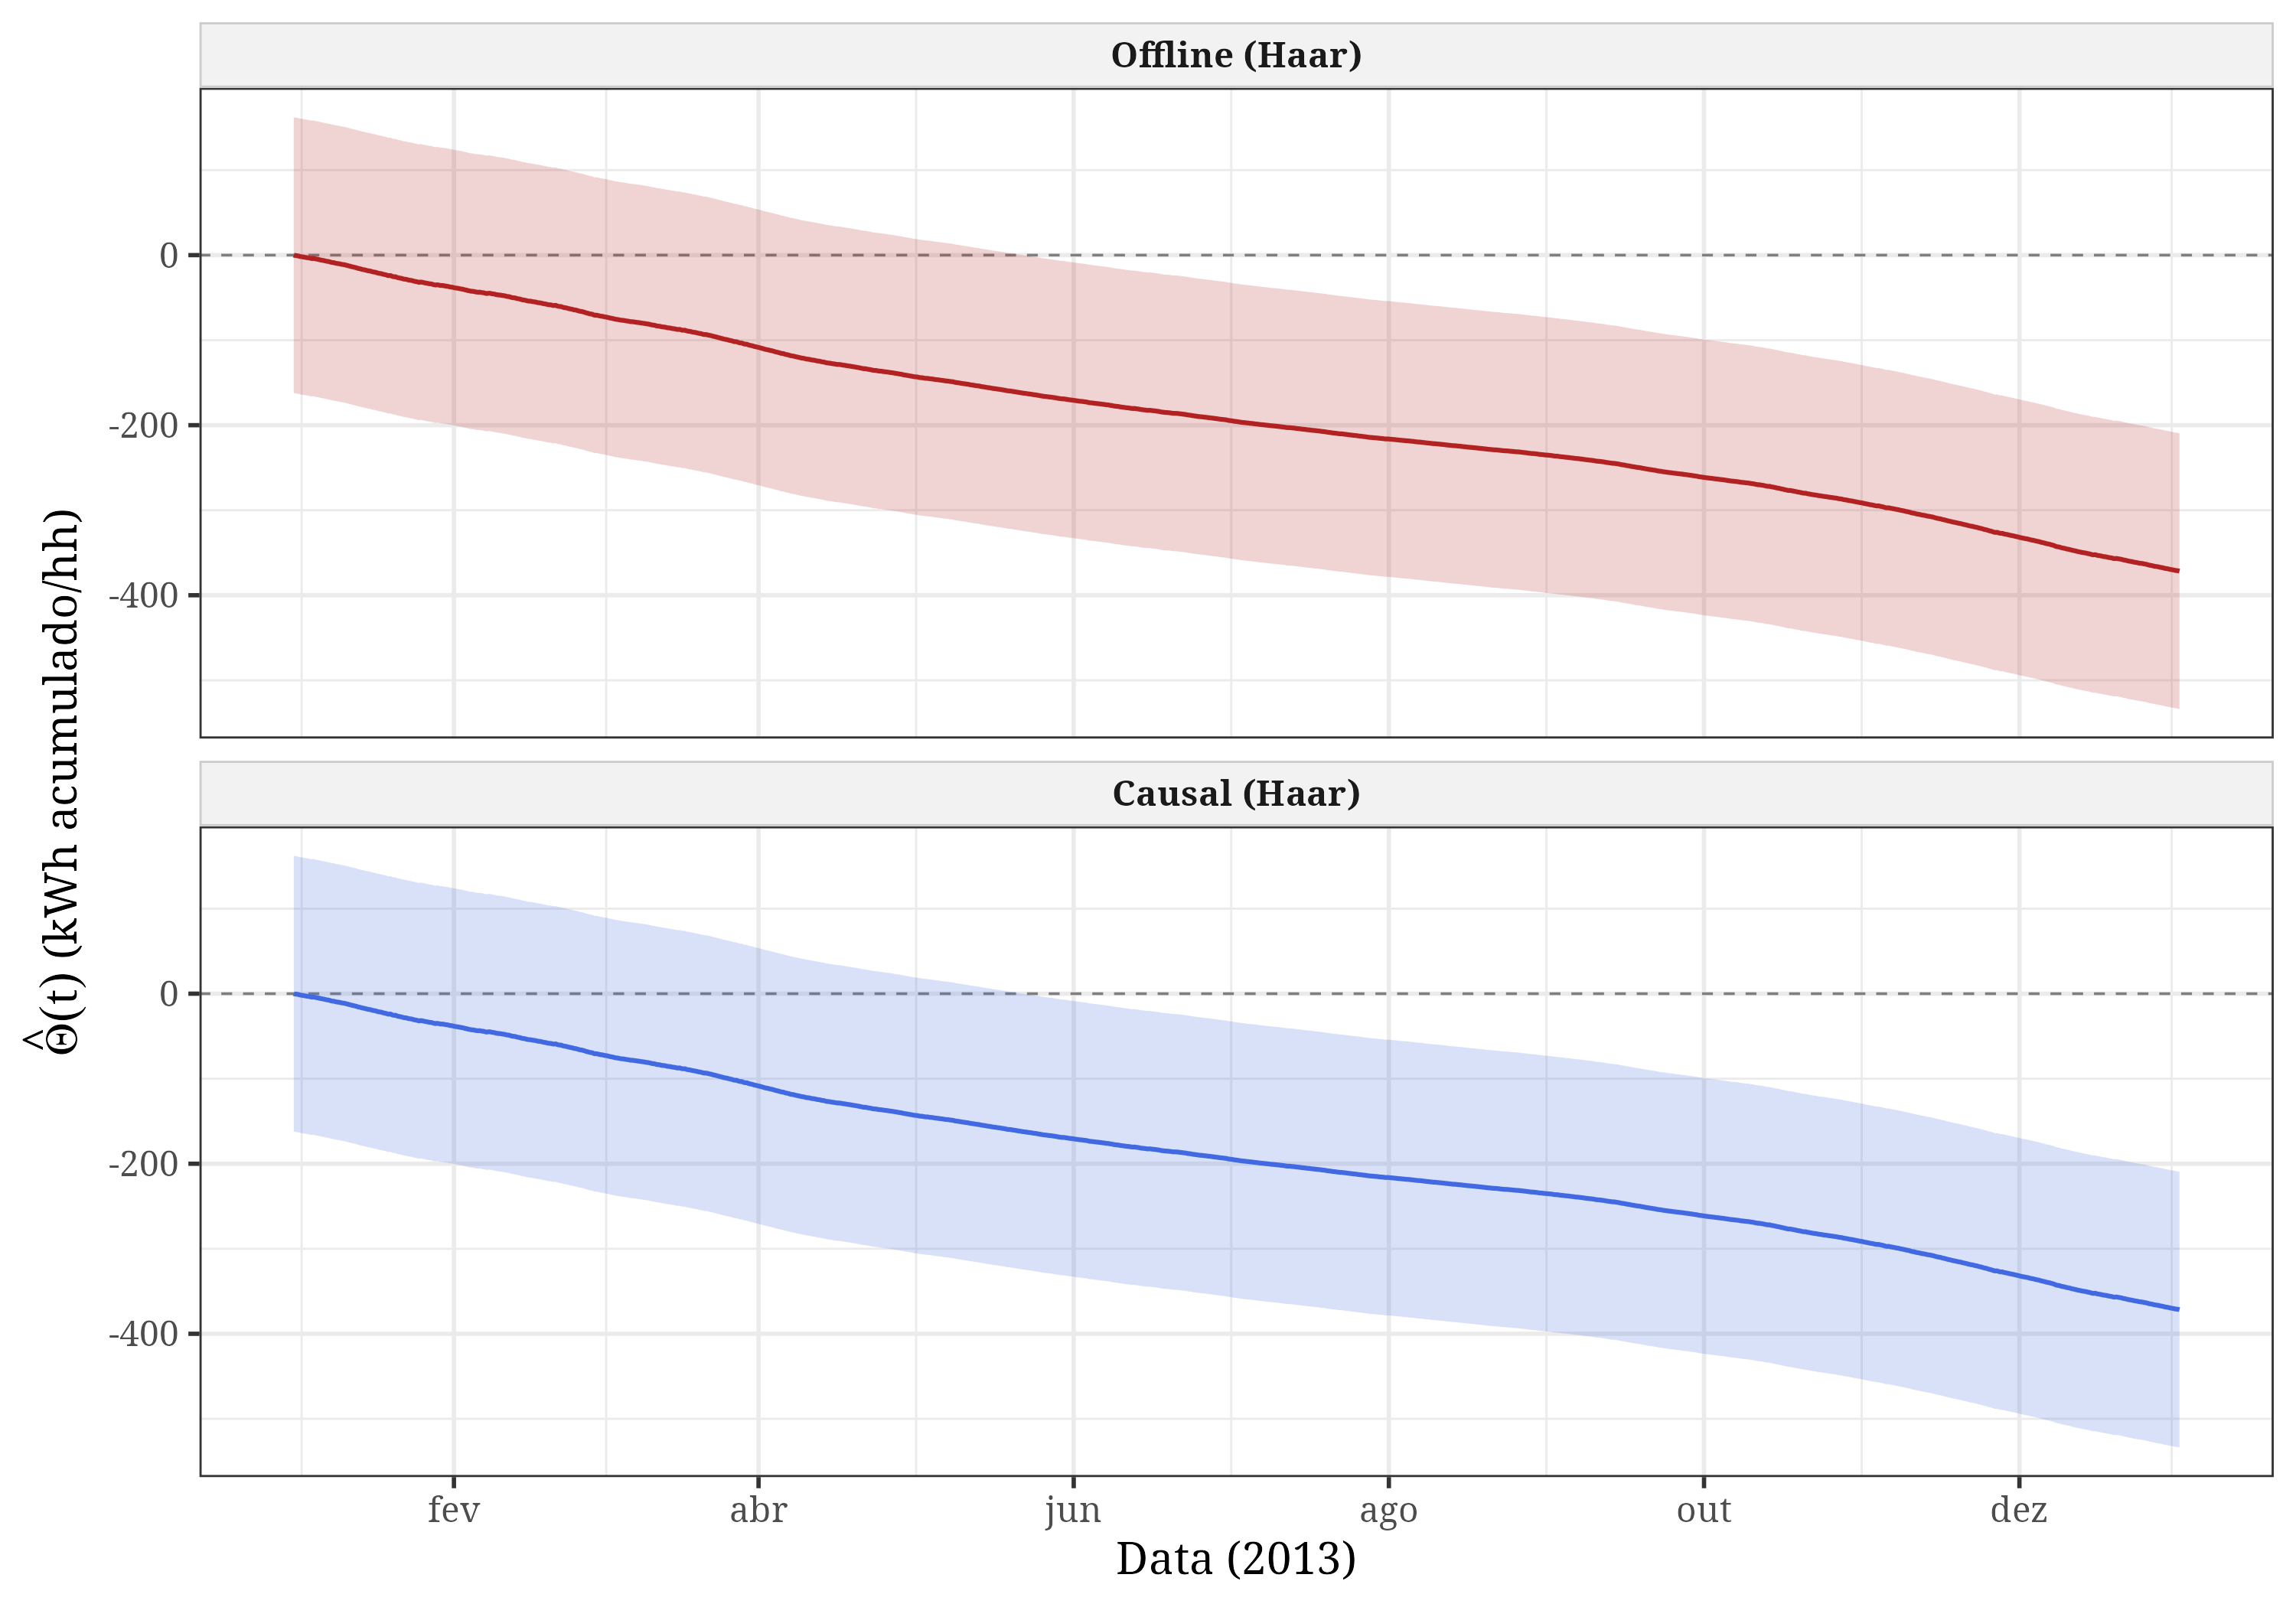
\includegraphics[width=0.9\textwidth]{../../fate-fda-application/low_carbon_energy/output/lcl_final/plots/main_text/cfate_annual}
    \caption{\(\mathrm{CFATE}\) acumulado ao longo de 2013 com bandas de confiança simultâneas a 95\%, nos modos \emph{offline} e \emph{online} (Haar). Valor final: \(-372\) kWh por domicílio [IC 95\%: \(-534\); \(-209\)].}
    \label{fig:lcl-cfate-anual}
\end{figure}

Avaliamos a heterogeneidade do efeito entre os grupos ACORN na Figura \ref{fig:lcl-fate-acorn-intradiario}.
Nela, apresentamos o perfil intradiário do \(\hat{\theta}(t)\) para cada grupo.
\emph{Affluent} e \emph{Comfortable} exibem redução em todos os horários, com queda mais acentuada no horário de pico.
\emph{Adversity} fica próximo de zero ao longo de todo o dia.
\emph{ACORN-U} é o único grupo com FATE positivo na maior parte do dia.
Os padrões coincidem com os da diferença bruta (Figura \ref{fig:lcl-diff-acorn-diario}), nos levando a crer que a heterogeneidade não é artefato do estimador.

\begin{figure}[htbp]
    \centering
    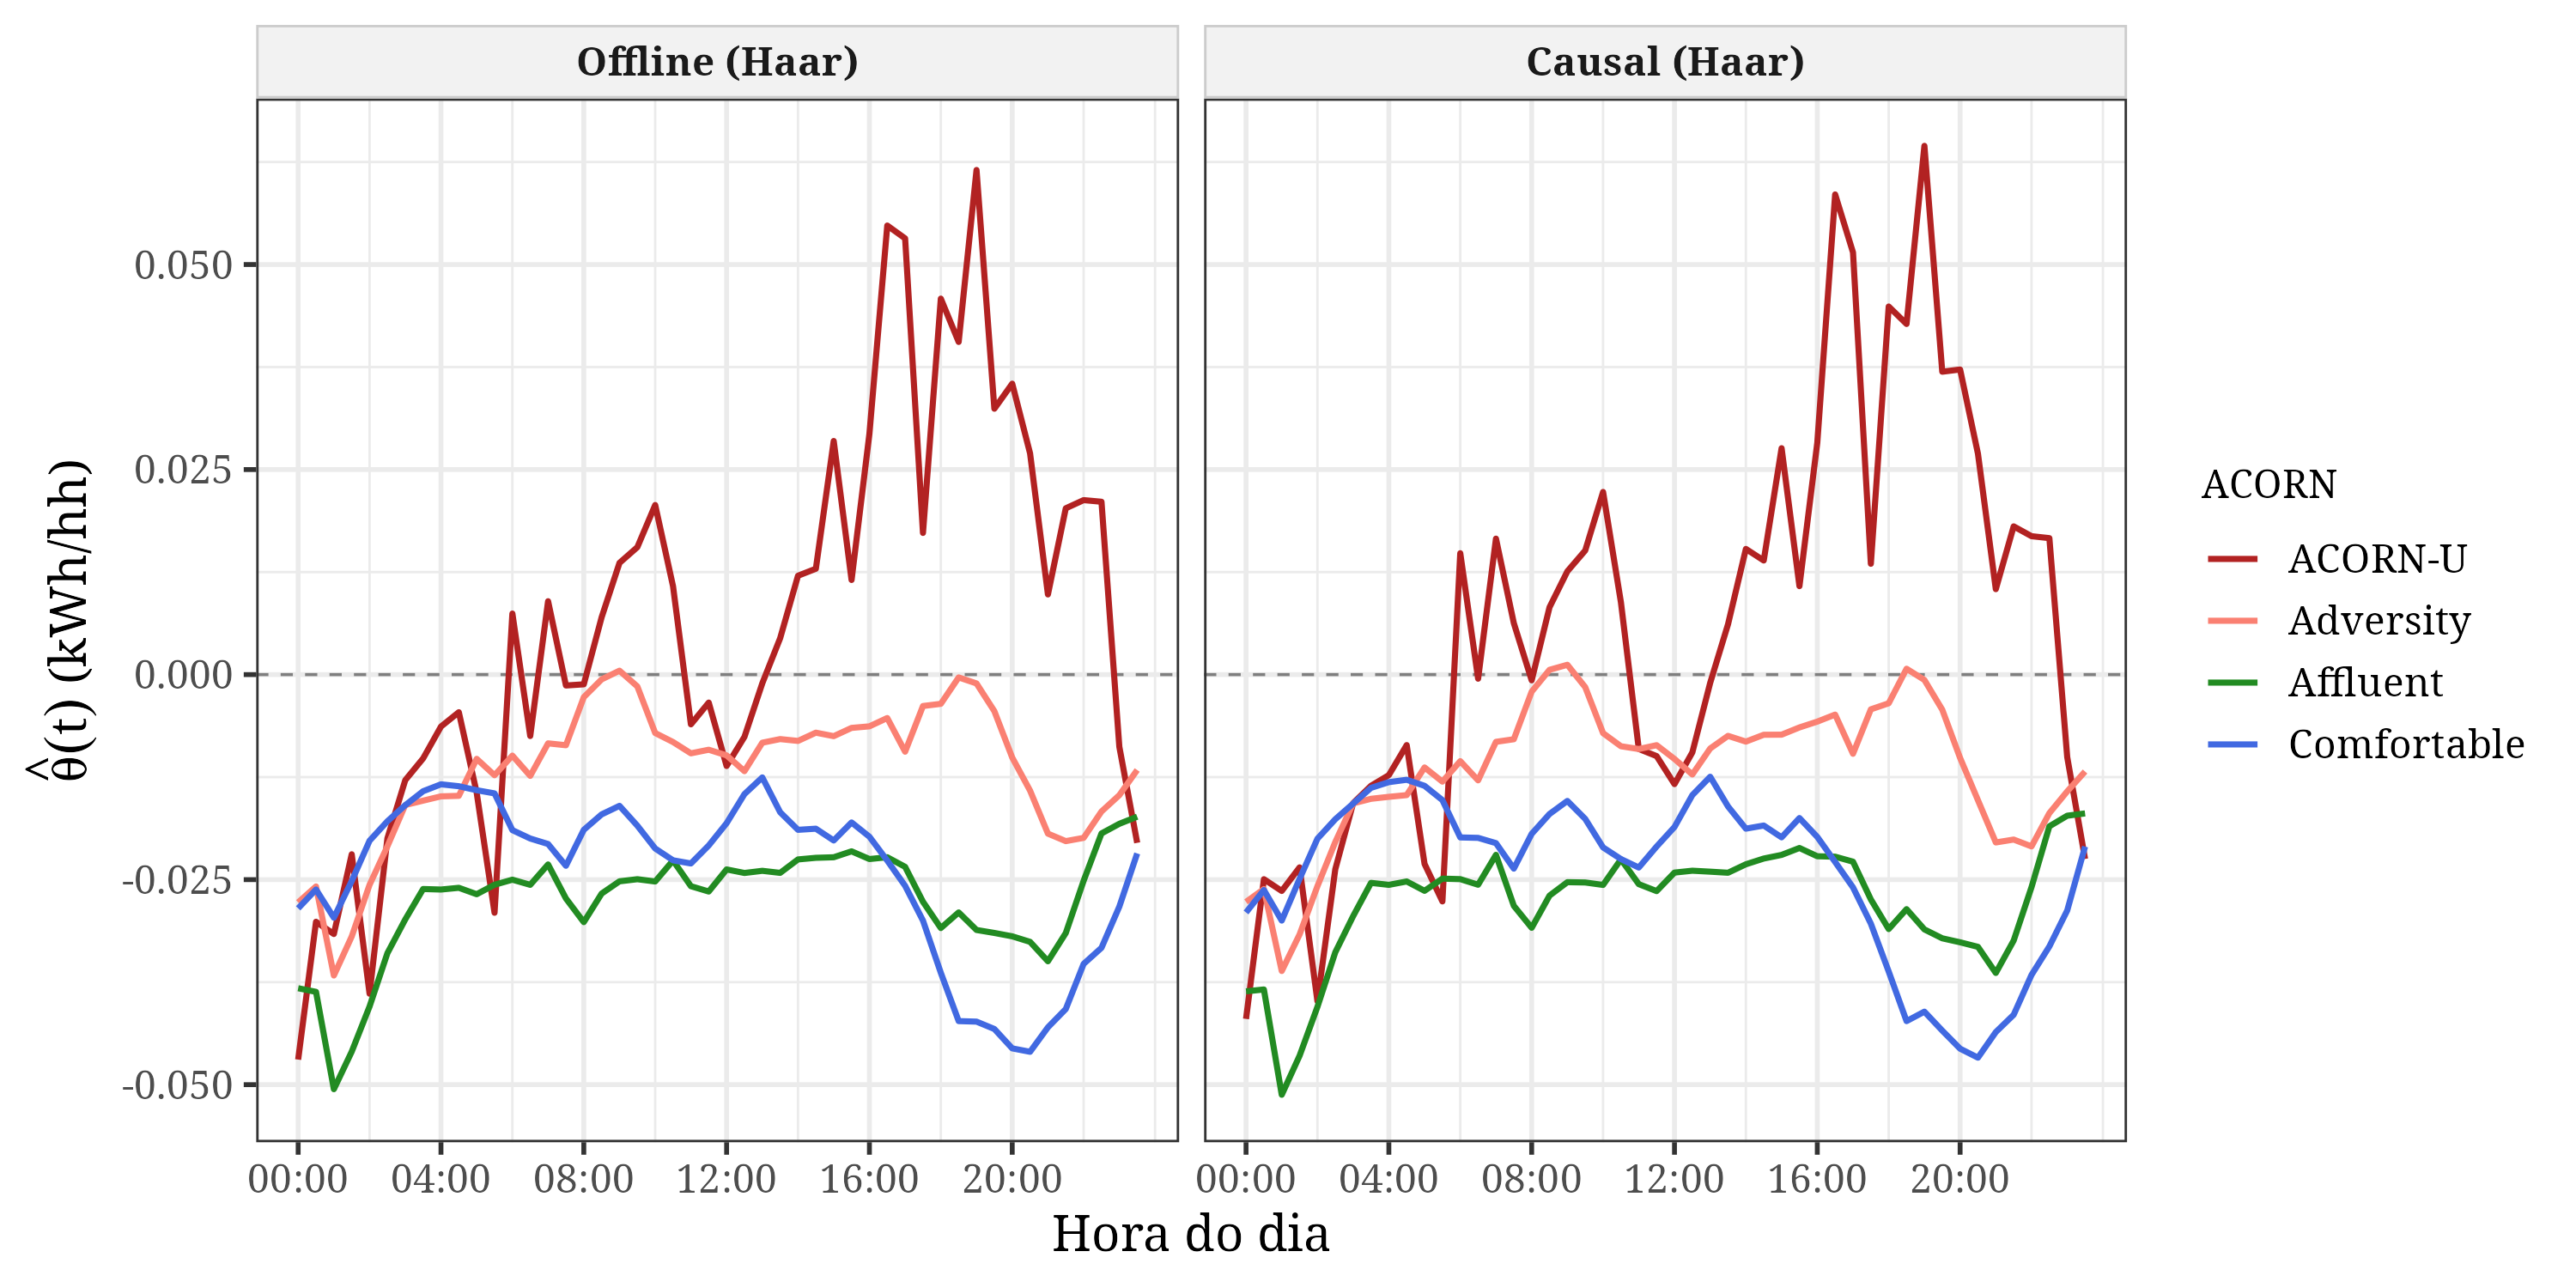
\includegraphics[width=0.9\textwidth]{../../fate-fda-application/low_carbon_energy/output/lcl_final/plots/main_text/fate_by_acorn_intraday}
    \caption{Perfil intradiário do \(\hat{\theta}(t)\) por grupo ACORN, estimativa \emph{offline} (Haar).}
    \label{fig:lcl-fate-acorn-intradiario}
\end{figure}

A Figura \ref{fig:lcl-cfate-acorn} apresenta o \(\mathrm{CFATE}\) acumulado por grupo.
\emph{Affluent} acumula a maior redução (\(-486\) kWh/hh), seguido de \emph{Comfortable} (\(-427\) kWh/hh) e \emph{Adversity} (\(-204\) kWh/hh).
\emph{ACORN-U} encerra o ano em \(+105\) kWh/hh.
A resposta à tarifa cresce com o nível de renda do grupo.
Reforçamos que os resultados de \emph{ACORN-U} devem ser interpretados com cautela, devido ao baixo tamanho de amostra deste grupo.

\begin{figure}[htbp]
    \centering
    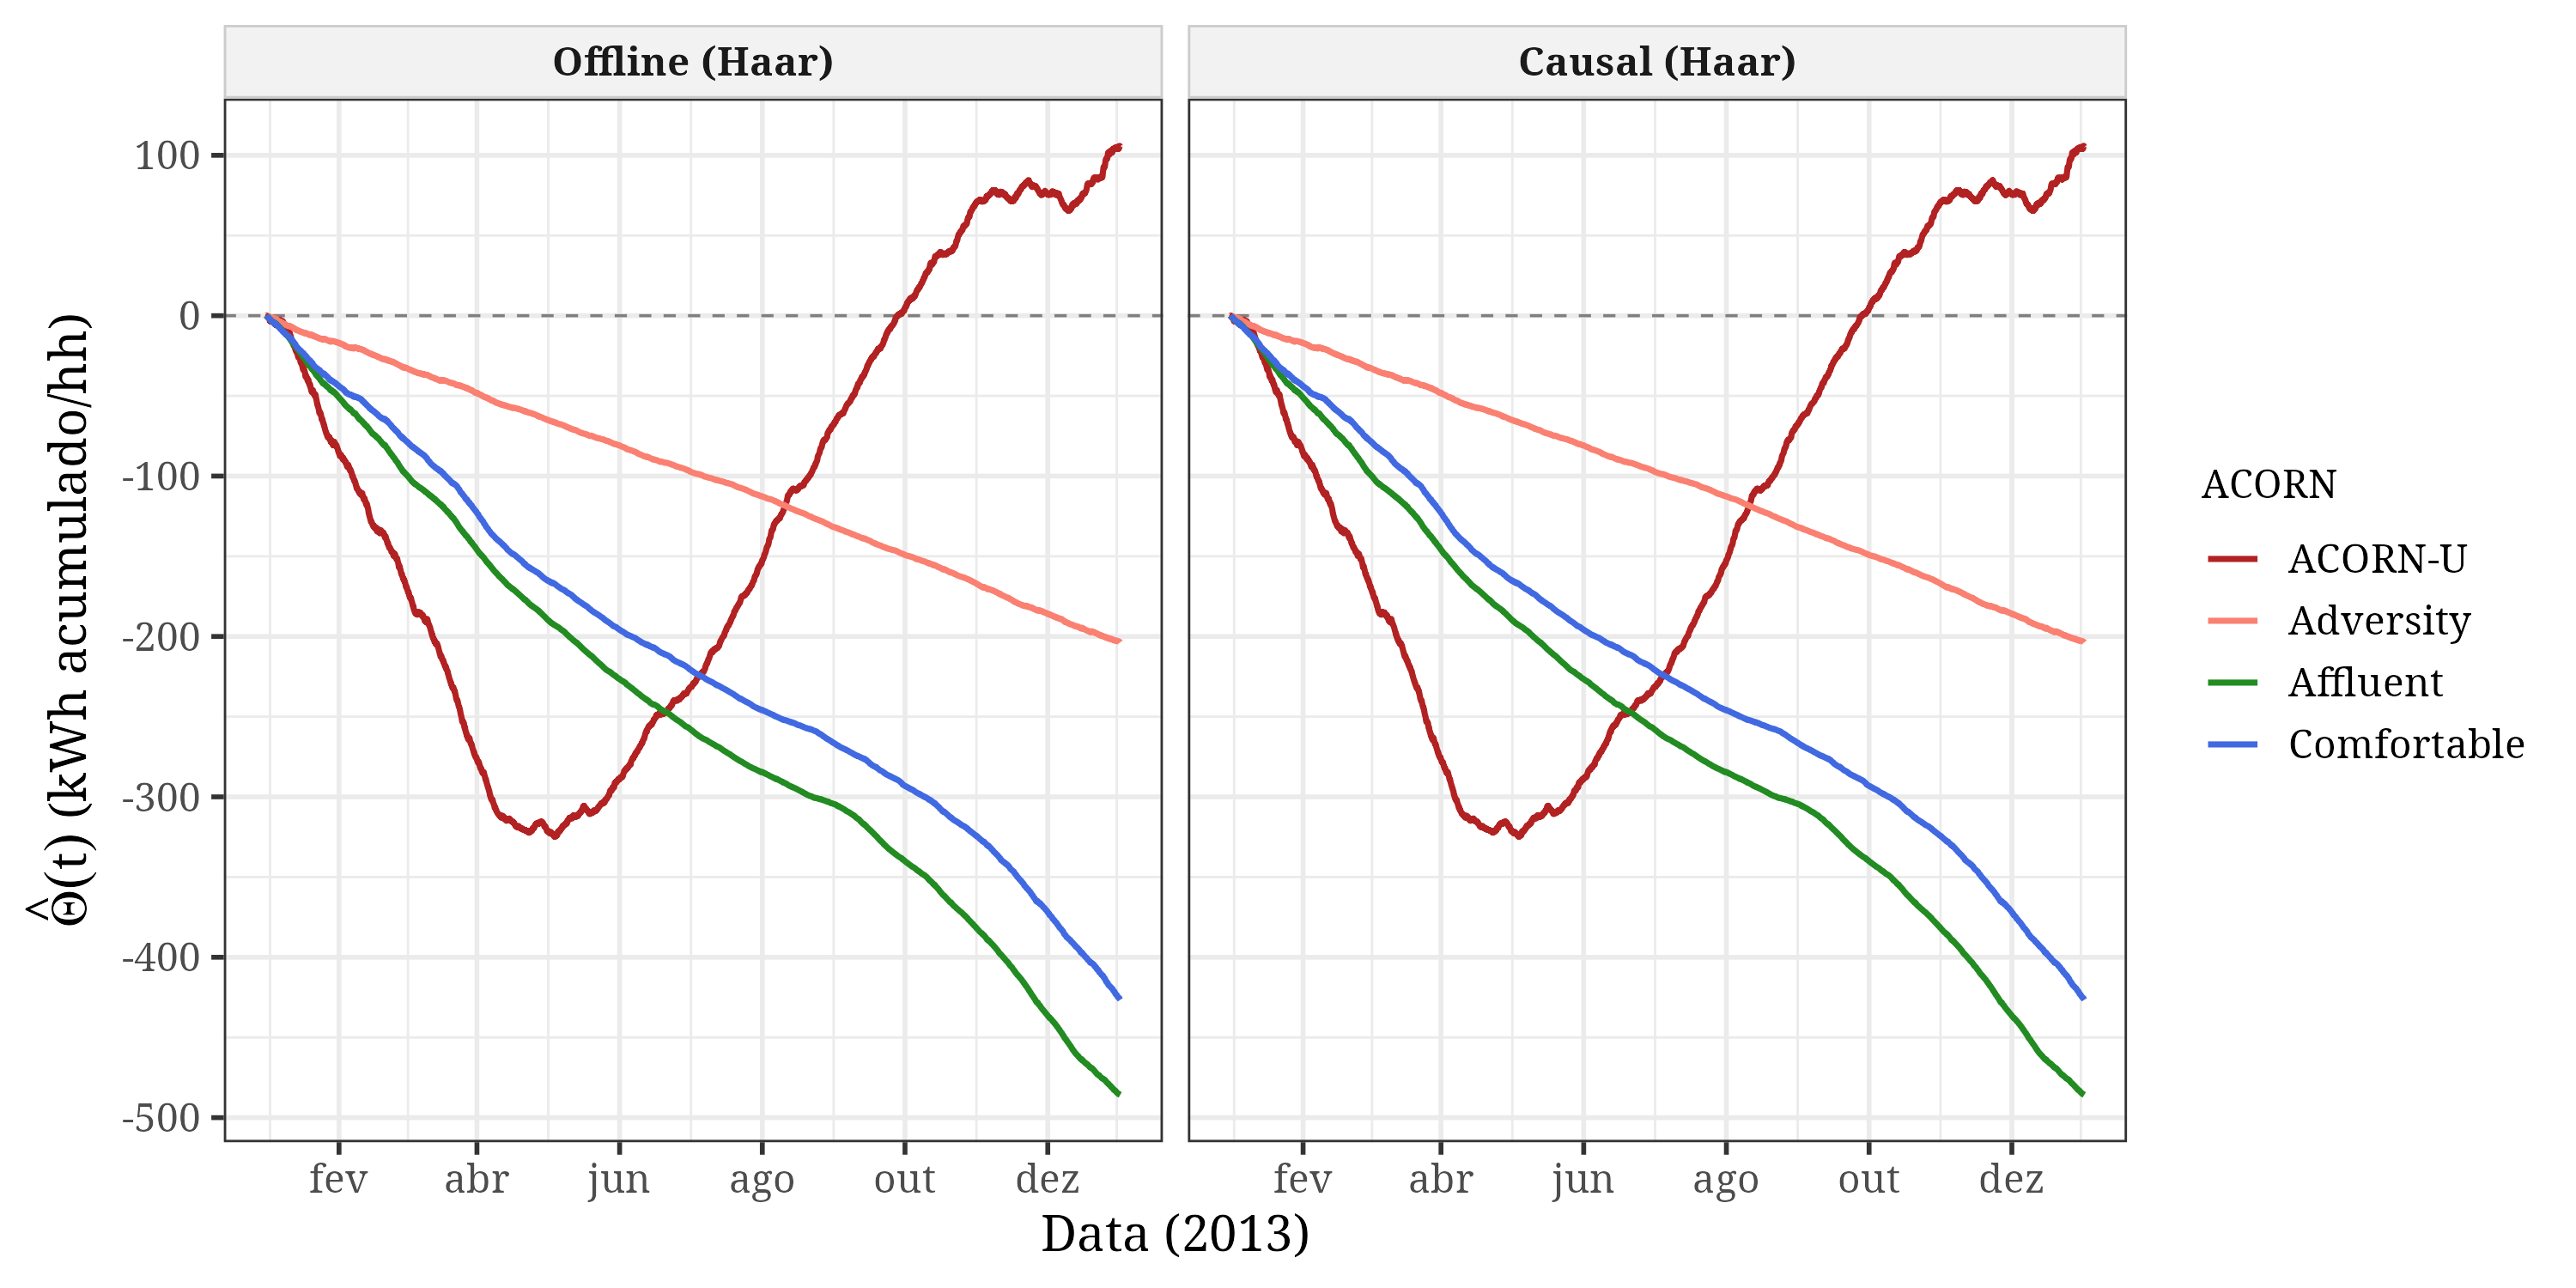
\includegraphics[width=0.9\textwidth]{../../fate-fda-application/low_carbon_energy/output/lcl_final/plots/main_text/cfate_by_acorn}
    \caption{\(\mathrm{CFATE}\) acumulado ao longo de 2013 por grupo ACORN, com bandas de confiança simultâneas a 95\%, modo \emph{offline} (Haar).}
    \label{fig:lcl-cfate-acorn}
\end{figure}

A Figura \ref{fig:lcl-sensitivity-sazonal} (Apêndice \ref{ap-aplicacoes}) desagrega o perfil intradiário do \(\hat{\theta}(t)\) por trimestre.
A forma qualitativa é preservada em todas as estações, com dois vales correspondentes à madrugada e ao horário de pico, e sem nenhum horário em que o efeito seja positivo.
A magnitude é maior no inverno e menor no verão.

Como verificação adicional, permutamos aleatoriamente os rótulos de tratamento entre os domicílios e recomputamos o \(\mathrm{FATE}\) em 200 iterações.
Quando os rótulos são permutados, o \(\mathrm{FATE}\) calculado oscila em torno de zero ao longo de todo o ano, enquanto a versão da Figura \ref{fig:lcl-fate-bandas}, estimada nos dados reais, permanece negativa neste período.
A Figura \ref{fig:lcl-sensitivity-placebo} (Apêndice \ref{ap-aplicacoes}) apresenta essa comparação.
